\subsection{Overall approach}
%[argument vs. current approaches start supporting performance of new resources by a more lenient apporach blb bla cut it]
%\kh{Guys, we really have to clarify the workding of 'performance': in performance-based remuneration, the 'performance' is a 'quality of execution' (Sect. 4.4 $\eta^{AS}$); however, our $\kappa$ does not look at 'performance' but rather at a 'quality of shape' (lacking a better word to describe the 'fitness' assessment quantified by $\kappa$.)}

%The key idea of the proposed approach is to formulate ideal performance requirements for each ancillary service in a number of relevant features, and then to provide a market mechanism that allows to define an optimal control resource portfolio building on beneficial combinations accounting for complementary properties of control resources. 
The proposed restructuring assumes that system operators acquire AS reserves through a market, and that potential AS providers bid their reserve capacity in that market. The restructuring is based on the following four key concepts (which are expanded upon throughout this section):
\begin{itemize}
    \item The formulation of an \emph{ideal ancillary service response} that the system operator desires for the system. This formulation will be strongly dependent on the needs of the system operator, e.g. very fast response in case of low system inertia, and will be submitted as a tender to the market.
    \item The \emph{parametrization of the AS bids}, where the parameters reflect the service providers' capabilities to partially fulfill the ideal service response. This removes the minimum-requirements-barriers on new technologies, thus enabling any useful unit to participate in the AS provision, which facilitates market liquidity.
    \item Clearing all units under a \emph{generalized single clearing-price auction}, provides incentives to bid actual marginal cost. In this auction, the capability value of each service provider and their historical performance is taken into account.
    \item \emph{Performance-based remuneration} gives incentive to better AS provision and enables transparent performance-based clearing of the market.
\end{itemize}
%to formulate an ideal tender requirements for each ancillary service, based upon a number of key parameters that directly address the system needs\bondy{fix}. Since current market mechanisms implicitly rely on a homogeneous set of responses, a proposal for a new market mechanism is presented, which allows to define an optimal control resource portfolio. The portfolio is built on optimal combinations of the resource key parameters, accounting for complementary properties of the resources, and seeks to minimize the cost of the reserve while ensuring that the overall response of the portfolio is optimal with respect to the service needs\bondy{fix to minimum capability tender}. 

%performance is thus embedded in present ancillary service definitions assumes only the exact following of the service is beneficial to the system - on the contrary actually resources may have dynamics that complement each other.
%essentially ...
%((linear) combination of heterogeneous portfolio)
%vs. 
%(scalar decomposition of homogeneous portfolio)

%ARGUMENTS:

%(1) The \textit{parametrization of AS bids} removes minimum requirements, enabling any 'useful' unit to participate (facilitates market liquidity, removing barriers for demand response participation);
%(2) A generalized \textit{single clearing-price auction}  providing incentives to bid actual marginal cost.
% REF for now: https://www.epsa.org/forms/documents/DocumentFormPublic/view?id=F64F00000033 and
%(3) \textit{Performance-based remuneration} incentivizes better service and enables transparent performance-based clearing;

Based on an assessment of the complete decision process, we merge the four key concepts outlined before into a novel approach to ancillary service valuation that accounts both for performance of resources and the actual spectrum of system needs.  % The actual market clearing is then
The holistic assessment includes:
\begin{itemize}
	\item \textit{Planning}: Assessment of system need, parametrization of resource performance and specification of tender conditions.

	\item \textit{Scheduling}: Quantification of AS tender volume, AS bid submission, and market clearing.

	\item \textit{Operation}: Reserves dispatch/activation and monitoring.

	\item \textit{Settlement}: Verification of service delivery and remuneration.
\end{itemize}

As outlined above, for effective inclusion of DR (or any other unconventional resource) in AS markets, a revision of each phase is required. Our proposal focuses on a new \textit{parametrization of services} (Sec.~\ref{subsec:parametrization}), which affects in particular \textit{market clearing} (Sec.~\ref{subsec:marketmechanism}) and \textit{remuneration} (Sec.~\ref{subsec:performanceremuneration}). 

In Section~\ref{sec:ddrascasestudy} we illustrate the impact of this reformulation in comparison with present market mechanisms, and in \ref{sec:ddrasdiscussion}, the alignment with present mechanisms and its applicability to novel ancillary service models (REF WARRINGTON/policy based) is reflected.  

\subsection{Ideal service tender}\label{subsec:idealtender}
The ideal source for AS is one with ``unlimited capabilities in terms of response time, energy output, ability to frequently reverse their output, ability to respond and follow the AGC setpoint changes, and size .''\cite{makarov2008assessing}\footnote{For this kind of response to be optimal, changes must be made to the AGC algorithm \cite{peydayesh2012effects}.} It is impossible for any one unit to possess these characteristics, but system operators aim at achieving this kind of system response by contracting several units.

In existing AS, there is an implicit assumption that ideal unit response corresponds to a scalar fraction of the required system response. In contrast, in presence of a diverse resource portfolio, the commonly expected fast response is secondary to an overall cheaper mixed portfolio which delivers a better system response, e.g. by combination of a fast duration-limited and slower unlimited response time resources.

%\kh{What is the difference between conventional dimensioning (see "operations manual") and dimensioning with capability parametrization?}

For example, a system operator could determine that the ideal system response to a frequency excursion is the one that has a resulting frequency nadir at the settling frequency (thus minimizing the risk of tripping the under-frequency relays). Based upon the inertia in its system, the system operator determines the volume ($V_{tot})$ needed as well as the response characteristics needed to achieve this, see Figure~\ref{fig:ddrasidealresponse}.

\begin{figure}[htbp!]
\centering
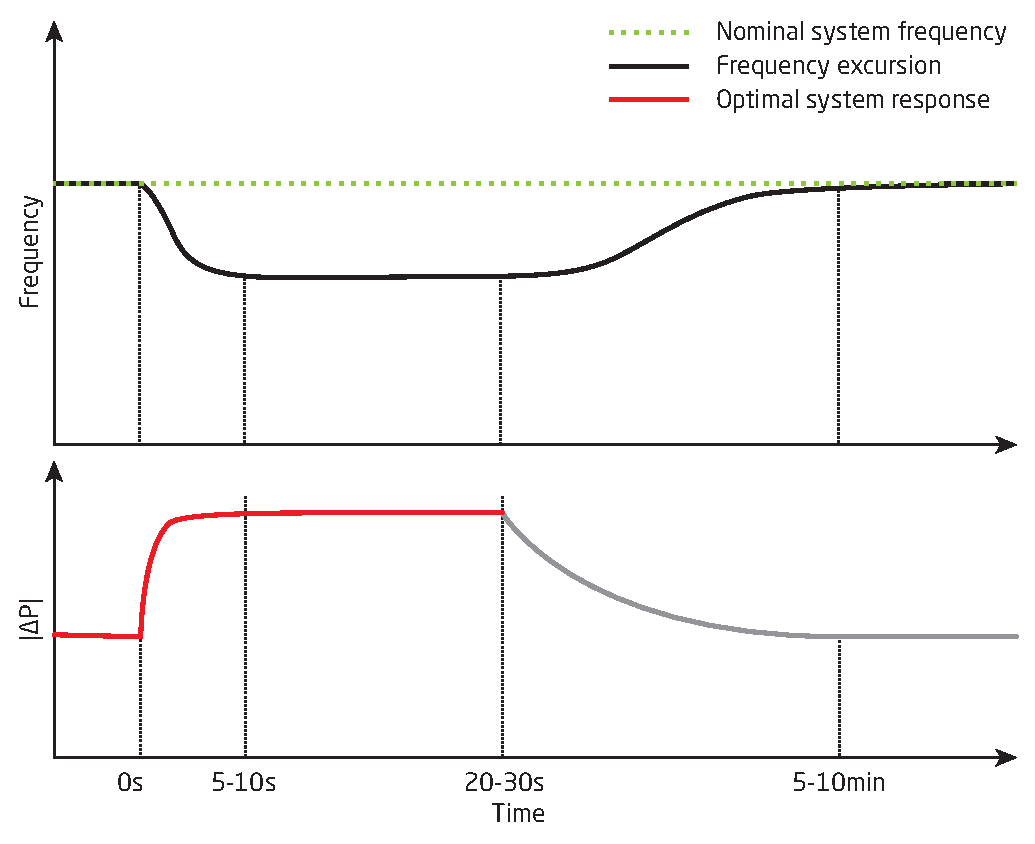
\includegraphics[width=1\columnwidth]{graphics/ddras/primary_frequency_control_ideal.eps}
\caption{In this case, the ramp of the ideal response is mainly determined by the system inertia and is to be sustained until secondary frequency control can be activated.}
\label{fig:ddrasidealresponse}
\end{figure}
%%4.2
%* bid formulation uses simplified constraints that can be addressed both for conventional generation and are also straightforward to be formulated as response capability of a diverse DR portfolio;

\subsection{Parametrization of service performance}\label{subsec:parametrization}

Ancillary service requirements are specified by a system operator based on the desired control response for a particular power system. Today, these requirements --- as reflected in the service definition --- are not differentiated according to the capabilities of the unit providing the service. Therefore, service definitions are designed to accommodate the least capable unit in the portfolio. As a consequence, more capable units are not being fully utilized, leading to excess contracting of service providers.
This suboptimal allocation of resources could be addressed by introducing a performance dependent definition of ancillary services, i.e. a service definition which allows compliance to be measured on a linear rather than a binary scale: In addition to compliance and noncompliance, different levels of partial compliance are possible.
In this context, services will be defined such that the best possible performance of the most capable unit corresponds to full compliance. The overall ideal service requirements can be expressed as:
\begin{equation}
	S^* = f_m(\textbf{x}^*) \label{eq:ddrasoptimaltender}
\end{equation}
where $\textbf{x}^*$ is a vector of ideal parameter values and $f_m(\cdot)$ a function that translates the parameters $\textbf{x}$ into a model. Furthermore, the system operator must inform how the parameters are valued with respect to the $S^*$, which is done through a capability value:
\begin{align}
    \kappa &= g(\mathbf{x}) \\
    \kappa &\in [0,1].
\end{align}

AS aggregator bids submitted include: 
\begin{itemize}
\item offered service parameters: $\mathbf{x}$
\item bid price: $P^{bid}$
\item (for cross-validation) estimated: $\kappa$
\item unit quantity (volume): \emph{V}
\end{itemize}

The bid parameters are service-specific and serve both for market-clearing and performance calculation. 

%%4.3
\subsection{Market mechanism}\label{subsec:marketmechanism}

In order to leverage the proposed AS restructuring, the market clearing mechanism needs to be changed. The clearing should take the \emph{capability value} of the service providers into account, and ideally also the probability of availability (certainty in service). There are many different ways of formulating such a market clearing mechanism and here we present an example of a market that utilizes the service parametrization to form an ideal service response.

The market is designed as a single clearing price auction, in which each resource bid is adjusted by \textit{two} factors for bid quality: 1) a shape-matching parameter $\kappa_i$ and 2) a historic performance  parameter $\eta^{hist}_i$.
%The benefit of the merit order is that by remuneration at clearing price it provides competitive incentive for bidding with true marginal cost 
The clearing mechanism identifies a common clearing price based on the most expensive accepted bid. 
%Clearing principles
\begin{equation}
    P^\mathtt{clear} = \max P^\mathtt{bid}_i, \quad i \in \Omega^\mathtt{acc}
\end{equation}
where $\Omega^{acc}\subseteq \Omega$ is the subset of accepted bids of the set of received bids $\Omega$. 
The clearing mechanism selects the subset of bids which offer the cheapest overall clearing cost and meet the tender requirements: 
\begin{align}
      \Omega^\mathtt{acc} &= &\mathtt{argmin}_{\Omega^\mathtt{hyp} \in \mathcal P(\Omega)} \sum_{i\in \Omega^\mathtt{hyp}}{\kappa_i P^\mathtt{clear}_{\Omega^\mathtt{hyp}} } & \\
      &\mathtt{s.t.}& \sum_{i\in \Omega^\mathtt{hyp}} V_{i}\ge V_{tot} &  \\
      &~ & \eta^{hist}_i \geq \eta^{hist}_{min} &\quad \forall i \in \Omega^\mathtt{hyp} \\
      &~ &\sum_{i\in \Omega^\mathtt{hyp}}{\eta_i V_i}/V_{tot} \geq \eta^{AS}& 
\end{align}
Where $\mathcal P(\Omega)$ denotes the Power Set of $\Omega$.
%As both tender specification and bid parametrization correspond to a $n$-dimensional polygons, the bids can be summed up and the sum can be compared to the tender polygon.

The specification of tender and bid parametrization needs to be aligned with the mechanisms applied during real-time operation the resource dispatch and activation.
Resource performance is monitored with respect to the behaviour expected from bid parametrization, and is further expanded upon in the next subsection.




%%4.4
\subsection{Performance-based remuneration}\label{subsec:performanceremuneration}
%\bondy{I write here}

%\bondy{3) adherence to performance model is evaluated and applied to base price}

Performance-based remuneration has already been introduced in United States through the FERC order 755. Similarly, in this work we propose that service providers are paid according to how close they follow the capability parameters they bid to the market. The estimation of the service provision performance can be done in different ways, depending on which parameters the system operator deems to be the most critical. A service performance index is proposed in \cite{bondy2016method}, where service performance is defined as the root mean square error of the actual service delivery compared to the ideal model:
 \begin{align}
     \eta^{post} &= \sqrt{\frac{\sum^{N}_{t=0} \left( {QoS_{t}}^{2} \right)}{N}},\\
     \eta^{post} & \in [0,1],
 \end{align}
 where \emph{N} is the time horizon over which the service is delivered and $QoS \in [0,1]$ is the \emph{Quality of Service} of the ancillary service, which is the error in service delivery scaled to the tolerance limits defined by the system operator. This leads to the final settlement price of service provision being defined as:
\begin{equation}
    P^\mathtt{rem}_i = \eta^{post}_i\kappa_i  P^\mathtt{clear} \qquad \forall i \in \Omega^\mathtt{acc}.
\end{equation}
 
